\documentclass[11pt,a4paper]{article}
\usepackage{fontspec}
\usepackage[french]{babel}
\usepackage{amsmath,amssymb}
\usepackage[margin=2.3cm]{geometry}
\usepackage{booktabs,longtable,tabularx,array}
\usepackage{graphicx}
\usepackage{enumitem}
\usepackage{xcolor}
\usepackage{microtype}
\usepackage{url}
\usepackage{hyperref}

\hypersetup{colorlinks=true,linkcolor=blue!45!black,urlcolor=blue!45!black}
\setlist{nosep}
\newcommand{\code}[1]{\texttt{#1}}
\newcommand{\NW}{\mathrm{NW}}
\graphicspath{{../figures/}}

\title{Étude de sensibilité M4B — rapport préliminaire\\
\large Audit, pilotes, exploration OAT et screening global ;
décisions avant la phase confirmatoire}
\author{Campagne \code{recherche/sensibilite\_m4b}}
\date{18 juillet 2026}

\begin{document}
\maketitle

\begin{abstract}
Ce rapport présente les résultats de la phase exploratoire de l'étude de
sensibilité du modèle de société de crédit M4B, conformément au protocole
figé du 17 juillet 2026 (\code{protocole.pdf}). Il couvre : l'audit du
moteur et l'inventaire des données existantes ; les cellules pilotes qui
auditent les plages de paramètres ; les contrôles de probité temporelle ;
les courbes un-facteur-à-la-fois (OAT) ; les sondes de frontière ; le
screening global sur plan hypercube latin ; et la carte d'extinction à
petite intensité de naissances. Il se conclut par la liste justifiée des
cellules confirmatoires et des coupes bidimensionnelles. Résultat
d'ensemble : dans toutes les plages auditées à $\lambda=30$, le modèle est
stationnaire, sans extinction ni censure par le garde-fou ; les réponses
sont continues ; la principale structure non linéaire est une transition
douce mais rapide dans la zone $\sigma\in[0,\,0{,}2]$ entre un régime de
cascades très propagatives ($b\simeq0{,}65$--$0{,}77$) et le régime de
plateau ($b\simeq0{,}30$) ; et la volatilité $\sigma$ domine la
démographie, tandis que $k$ domine les inégalités et la statistique fine
des avalanches, $K_0$ agit log-linéairement sur la durée de vie et
$\delta$ se comporte surtout comme une échelle du capital.
\end{abstract}

\tableofcontents

\section{Rappels et conventions}

Le modèle, ses paramètres ($\lambda$ intensité des naissances, $\delta$
dépréciation, $\sigma$ volatilité du choc multiplicatif, $K_0$ capital de
naissance, $k$ taille de l'échantillon du marché local), le dictionnaire
des métriques et les règles d'analyse sont définis dans le protocole
(\code{report/protocole.pdf}) ; les définitions essentielles sont
rappelées au fil du texte. Sauf mention contraire : horizon $T=2000$,
fenêtre d'analyse $[T/4,\,T]$, graines d'exploration $\{1,2,3\}$
partagées entre cellules (contrastes appariés), écriture minimale
(neutralité démontrée, section~\ref{sec:audit}). Toutes les cellules
citées sont identifiées par leur \code{run\_id} dans les manifestes
(\code{manifests/*.json}) ; l'annexe~\ref{sec:annexe} donne la
correspondance des cellules citées.

Le rapport distingue systématiquement : \emph{fait simulé} (valeur lue
dans les données d'un run), \emph{inférence statistique} (estimation avec
incertitude) et \emph{hypothèse} (interprétation à confirmer).

\section{Audit du moteur et des données}
\label{sec:audit}

Réalisé le 17 juillet 2026, détails dans le protocole
(section « Audit ») et le journal (\code{JOURNAL.md}) :

\begin{itemize}
\item 6/6 tests du moteur passés, dont la parité exacte M4/M4B champ par
  champ sur deux régimes — unique recours exécutable à M4 de l'étude ;
  4/4 tests des routines statistiques passés ;
\item neutralité des options de mesure : séries bit à bit identiques
  entre écriture minimale et complète (deux contrôles) ;
\item intégrité comptable : résidu relatif maximal $6\cdot10^{-16}$ sur
  les runs de benchmark, zéro erreur de carnet ; ce contrôle est répété
  sur chaque run de campagne (aucune violation à ce jour) ;
\item provenance : moteur \code{m4b-mini-3}, condensat
  \code{f3a7ce02cd9185c7}, inscrit dans chaque manifeste ;
\item inventaire : aucun run M4B préexistant réutilisable (10 runs de
  validation d'intégration dans Simulation Lab, horizons courts, panels
  non contrôlés) — la campagne reproduit tout sous manifeste.
\end{itemize}

\section{Pilotes : audit des plages initiales}
\label{sec:pilotes}

Trente cellules pilotes (plan \code{pilotes}, graines $\{1,2\}$) ont
couvert les coins de l'espace
$(\delta,\sigma)\in\{0{,}02;0{,}10\}\times\{0{,}10;0{,}50\}$, les
extrêmes $K_0\in\{5,100\}$ et $k\in\{2,10\}$, les contrôles $\sigma=0$,
le coin de mortalité $(K_0{=}5,\sigma{=}0{,}50,\delta{=}0{,}10)$, le
centre, et les contrôles temporels ($T=4000$ au centre, $T=8000$ au coin
lent, $\lambda=100$ au coin lent).

\paragraph{Résultat principal.} Les 30 runs terminent en statut
\code{ok} : aucune extinction, aucune censure par \code{pop\_max},
dérives relatives de population $\le 4\,\%$ sur la fenêtre, moitiés de
fenêtre cohérentes. \textbf{Les plages initiales sont donc validées sans
révision} : chaque coin produit un régime stationnaire non trivial, avec
des avalanches en effectif suffisant pour les ajustements
($\ge 3\,000$ événements de taille $\ge2$ par run partout).

\paragraph{Le contrôle $\sigma=0$ n'est pas dégénéré.} Fait simulé
inattendu : sans choc, le système reste mortel et stationnaire, avec une
population dense ($N/\lambda=36{,}9$--$37{,}0$ ; $46{,}2$--$46{,}7$ si
$\delta=0{,}02$) et des cascades très propagatives (rapport de
branchement $b=0{,}65$--$0{,}77$, exposant $\hat\alpha=1{,}72$--$1{,}80$,
Gini du capital $0{,}03$--$0{,}04$). Hypothèse mécanique (à documenter au
rapport final) : l'hétérogénéité par l'âge suffit — les jeunes
emprunteuses à faible $K$ contractent des dettes dont le service peut
excéder leur capital du pas, et l'insolvabilité par perte de créance
propage ensuite. Ce régime « corrélé » constitue une limite singulière
utile, conservée comme cellule confirmatoire.

\paragraph{Régimes lents déjà stationnaires.} Le coin
$(\delta{=}0{,}02,\sigma{=}0{,}10)$ donne $N/\lambda=24{,}1$--$24{,}4$ à
$T=2000$ et $24{,}3$ à $T=8000$ (dérive $\sim0$) : pas de transitoire
long dans les plages retenues ; les horizons $T\gg10^4$ envisagés par
prudence ne sont pas nécessaires ici.

\section{Contrôles de probité temporelle}
\label{sec:temps}

\begin{itemize}
\item \textbf{Horizon} : au centre, $T=4000$ reproduit $T=2000$ :
  $N/\lambda=14{,}8$ identique, $\hat\alpha$ $2{,}25$--$2{,}26$ contre
  $2{,}26$--$2{,}27$, $b=0{,}30$ stable, effectif de queue doublé
  ($\approx11\,300$).
\item \textbf{Burn-in} : sur les 30 pilotes, remplacer le burn-in $T/4$
  par $T/8$ ou $T/2$ change la population moyenne d'au plus $0{,}8\,\%$
  (médiane $0{,}2$--$0{,}3\,\%$), $\hat\alpha$ d'au plus $0{,}014$ et $b$
  d'au plus $0{,}004$ : le choix du burn-in est sans conséquence dans les
  plages explorées.
\item \textbf{Demi-fenêtres} : les écarts de population entre les deux
  moitiés de la fenêtre par défaut restent $\le4\,\%$ en relatif
  (généralement $\le2\,\%$), sans biais de signe systématique.
\end{itemize}

Conclusion (inférence) : les métriques fenêtrées de l'exploration sont
insensibles aux choix de fenêtre ; $T=2000$ suffit au screening, et le
passage à $T=4000$ en confirmation sert à doubler l'effectif des queues,
pas à corriger un biais temporel.

\section{Courbes OAT autour du centre}
\label{sec:oat}

Plan \code{oat} : 22 cellules uniques le long des cinq axes, graines
$\{1,2,3\}$, centre $\lambda=30$, $\delta=0{,}05$, $\sigma=0{,}25$,
$K_0=25$, $k=3$. Figures \path{figures/oat_<axe>.png} ; contrastes
appariés (cellule $-$ centre, même graine) dans
\path{results/summary/oat_contrasts.csv}.

\subsection{Volatilité $\sigma$ : levier dominant et transition douce}

\begin{figure}[tbh]
\centering
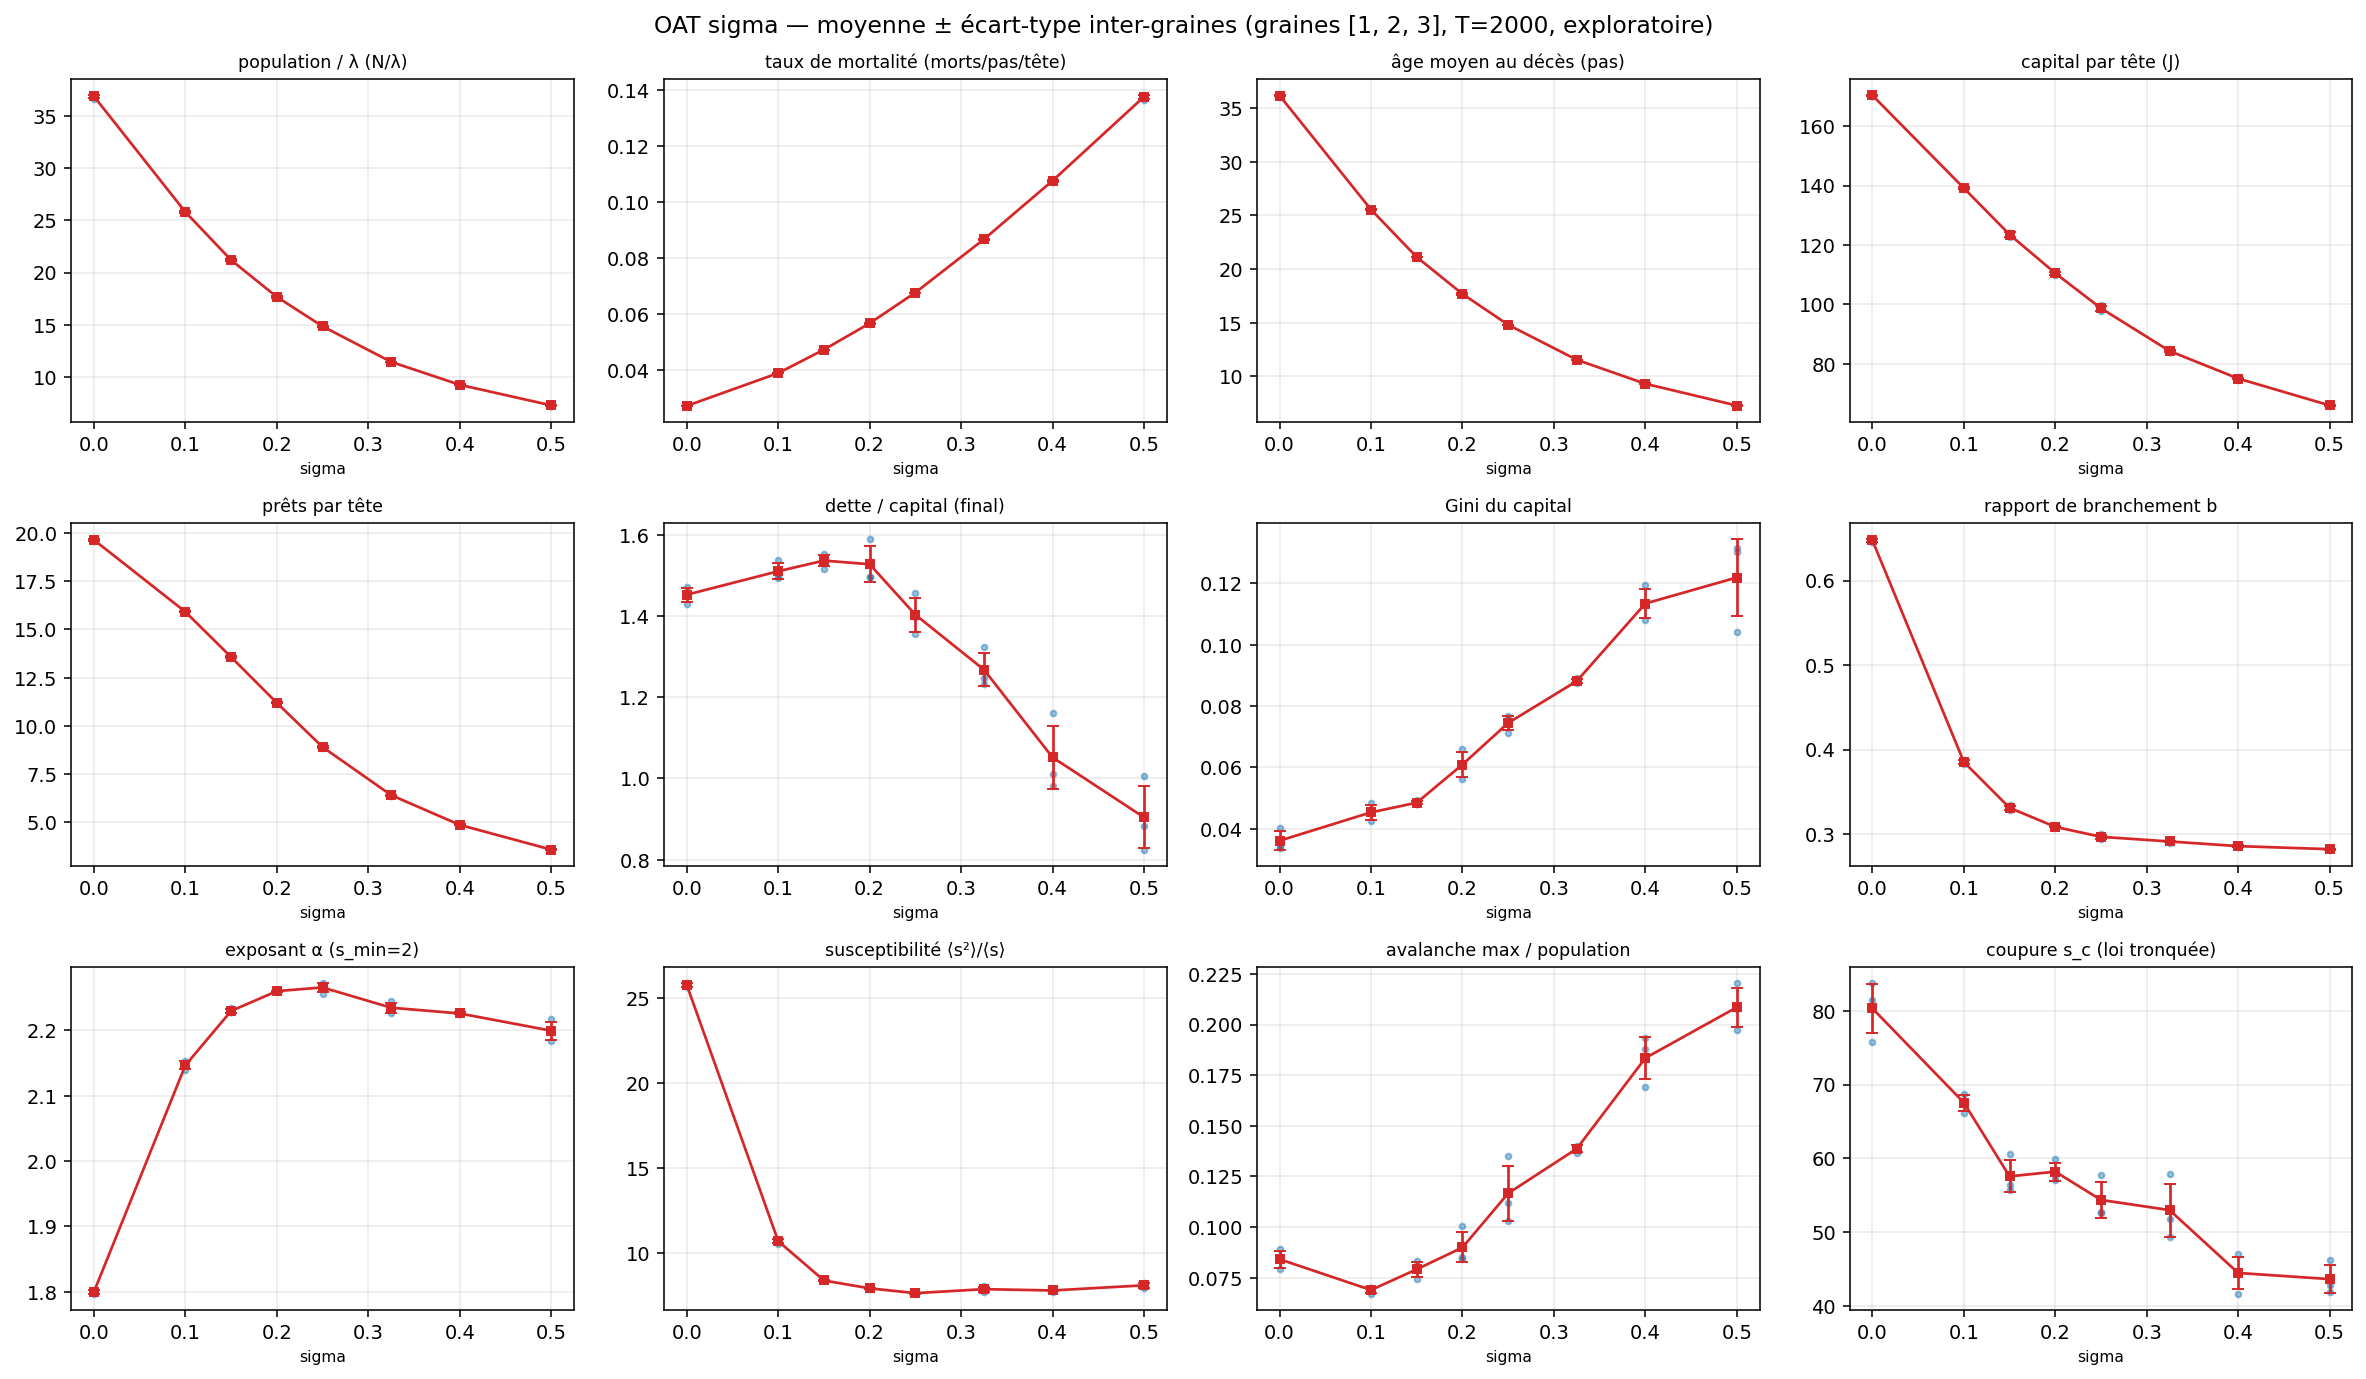
\includegraphics[width=\textwidth]{oat_sigma.png}
\caption{OAT $\sigma$ (12 métriques). Points bleus : graines ; carrés
rouges : moyenne $\pm$ écart-type inter-graines. Axe $\sigma$ de 0 à
0{,}5 ; le contrôle $\sigma=0$ est inclus comme limite.}
\label{fig:oat-sigma}
\end{figure}

Faits simulés (figure~\ref{fig:oat-sigma}) :

\begin{itemize}
\item $N/\lambda$ décroît de façon monotone et convexe : $36{,}9$
  ($\sigma=0$) $\to$ $14{,}9$ ($0{,}25$) $\to$ $7{,}2$ ($0{,}5$) ; le
  taux de mortalité croît convexement ($0{,}027\to0{,}138$ par tête et
  par pas). Prolongé par les sondes de frontière
  (section~\ref{sec:frontiere}) jusqu'à $N/\lambda=3{,}5$ à $\sigma=1$,
  toujours sans effondrement discontinu.
\item Toute la structure non linéaire de la propagation se concentre dans
  $\sigma\in[0,\,0{,}2]$ : $b$ chute de $0{,}65$ à $0{,}31$ puis reste
  quasi constant ($0{,}28$--$0{,}30$) ; la susceptibilité passe de $26$ à
  $8$ puis stagne ; $\hat\alpha$ monte de $1{,}80$ à $\simeq2{,}25$ puis
  plafonne.
\item La dette rapportée au capital est \textbf{non monotone} : maximum
  $\simeq1{,}53$ vers $\sigma\simeq0{,}15$--$0{,}2$, puis décroissance
  vers $0{,}90$ à $\sigma=0{,}5$. Hypothèse : à faible $\sigma$ le
  carnet survit longtemps (durées de vie longues) mais les écarts de
  capital qui motivent les prêts sont petits ; à fort $\sigma$ le carnet
  est détruit trop vite ; l'exposition maximale se situe entre les deux.
\item Le Gini du capital croît continûment avec $\sigma$
  ($0{,}036\to0{,}12$), de même que l'avalanche maximale rapportée à la
  population.
\end{itemize}

\subsection{Dépréciation $\delta$ : essentiellement une échelle du capital}

Faits simulés (\code{oat\_delta.png}) : $K$ par tête passe de $159$ à
$51$\,J quand $\delta$ va de $0{,}02$ à $0{,}10$ ; $N/\lambda$
\emph{augmente} de $13{,}5$ à $16{,}9$ (effet contre-intuitif mais très
net : écart-type inter-graines $\sim0{,}04$) ; la dette/capital décroît
($1{,}52\to1{,}17$) ; la statistique d'avalanches est à peine modifiée
($b$ : $0{,}299\to0{,}289$ ; $\hat\alpha$ : $2{,}29\to2{,}22$ ;
susceptibilité : $7{,}4\to8{,}1$). Hypothèse d'interprétation : $\delta$
fixe surtout l'échelle du capital individuel
($K^\ast=(1/\delta)^2$ pour l'équilibre production--dépréciation d'une
entité isolée), ce qui renormalise les taux du marché
($r_x=1/(2\sqrt{K_x})$) sans changer la topologie de propagation ; la
hausse de $N/\lambda$ avec $\delta$ (durée de vie plus longue à capital
plus faible) devra être expliquée au rapport final. $\delta$ est le
premier candidat au statut de « convention d'échelle » pour la
discussion de réduction.

\subsection{Capital de naissance $K_0$ : log-linéaire sur la survie}

Faits simulés (\code{oat\_K0.png}) : $N/\lambda$ croît de $10{,}7$ à
$19{,}9$ quand $K_0$ va de 5 à 100 (quasi linéaire en $\log K_0$) ; la
mortalité baisse d'un tiers ; $b$ est quasi plat
($0{,}296$--$0{,}306$) ; $\hat\alpha$ décroît modérément
($2{,}30\to2{,}14$) ; la susceptibilité monte ($6{,}9\to9{,}5$). La
dette/capital présente une bosse vers $K_0\simeq50$. $K_0$ agit donc
principalement sur la démographie (protection des jeunes) avec un effet
secondaire sur les queues.

\subsection{Taille du marché $k$ : inégalités et statistique fine}

Faits simulés (\code{oat\_k.png}) : la démographie est presque
insensible ($N/\lambda$ : $15{,}4\to14{,}5$), mais : Gini du capital
$0{,}136\to0{,}010$ ($k=2\to10$) ; $b$ décroît linéairement
$0{,}305\to0{,}237$ ; $\hat\alpha$ croît $2{,}21\to2{,}43$ ;
susceptibilité $8{,}3\to5{,}2$ ; dette/capital maximale à $k=4$
($1{,}44$). Interprétation (hypothèse) : un plus grand échantillon
sélectionne des paires plus contrastées, homogénéise le capital
(les cibles $K^\ast=\sqrt{K_\ell K_b}$ resserrent la distribution) et
fragmente l'exposition, d'où des cascades plus petites et une queue plus
raide.

\subsection{Axe de taille $\lambda$ : intensivité et coupure}

Faits simulés (\code{oat\_lam.png}) : $N/\lambda$, l'âge au décès, le
capital par tête, le Gini et la dette/capital sont stables à
$\pm2\,\%$ entre $\lambda=10$ et $100$ (grandeurs intensives) ; la
susceptibilité croît fortement avec la taille ($4{,}8\to15{,}4$) et le
maximum relatif décroît — signatures de taille finie attendues. À
$\lambda=100$, l'ajustement en loi tronquée dégénère (coupure estimée
$\sim10^8$, hors de la portée observable) tandis que le test de Vuong
bascule en faveur de la loi de puissance pure ($z=+15{,}0$ contre
$z=-6{,}5$ à $\lambda=10$ et $-4{,}2$ à $\lambda=30$) : la coupure de
taille finie sort de la fenêtre d'observation quand le système grandit.
Convention adoptée : lorsque $\hat s_c$ dépasse largement la plus grande
avalanche observée, la coupure est déclarée « au-delà de la portée
observable » et sa valeur numérique n'est pas interprétée.
$\hat\alpha(\lambda)$ présente une légère non-monotonie
($2{,}32/2{,}27/2{,}31$ pour $\lambda=10/30/100$) que la phase
confirmatoire devra trancher.

\subsection{Puissance statistique}

Au centre, les coefficients de variation inter-graines valent :
$0{,}1$--$1\,\%$ pour les moyennes démographiques et de propagation
($N/\lambda$, âge au décès, $b$, susceptibilité, $\hat\alpha$),
$3$--$5\,\%$ pour le Gini, la coupure et la dette/capital, $14\,\%$ pour
l'avalanche maximale. Avec 3 graines, l'effet minimal détectable
(à $2$ écarts-types du contraste apparié) est par exemple $0{,}06$ sur
$N/\lambda$, $0{,}005$ sur $b$, $0{,}014$ sur $\hat\alpha$ — très
inférieur aux effets observés le long des axes. Les 5 graines de la
confirmation sont surtout utiles aux métriques extrêmes (maximum,
coupure) et aux voisinages des non-monotonies.

\section{Sondes de frontière et carte d'extinction}
\label{sec:frontiere}

\subsection{Au-delà des plages, à $\lambda=30$}

Plan \code{pilotes2} (16 runs) : $\sigma\in\{0{,}6;0{,}7;0{,}85;1{,}0\}$,
$\delta=0{,}01$, $K_0\in\{2,200\}$. Tous \code{ok}. La durée de vie
moyenne décroît continûment jusqu'à $N/\lambda=3{,}5$ à $\sigma=1$
(mortalité $0{,}286$ par tête et par pas) sans transition brutale ni
extinction. Fait de structure : à $\lambda=30$, l'extinction absorbante
(population nulle en fin de pas) est pratiquement inaccessible, car
$P[\mathrm{Poisson}(30)=0]\approx10^{-13}$ : la « frontière
d'extinction » du modèle est une propriété du petit $\lambda$, pas des
paramètres microscopiques seuls.

\subsection{Carte d'extinction à petit $\lambda$}
\label{sec:lambdaext}

Plan \code{lambda\_ext} : $\lambda\in\{1,2,3,5,10\}\times
\sigma\in\{0{,}25;0{,}5;1{,}0\}$, 3 graines, 45 runs.

Faits simulés : les seules extinctions observées (9 runs sur 45 —
deux graines sur trois à $\lambda=1$ et une sur trois à $\lambda=2$,
identiques pour chaque $\sigma$ puisque l'événement ne dépend que du
premier tirage de Poisson) surviennent toutes au \emph{premier pas},
pour $\lambda\in\{1,2\}$ :
la population initiale étant vide, l'extinction se produit si le premier
tirage de Poisson est nul, événement de probabilité $e^{-\lambda}$
($0{,}37$ à $\lambda=1$, $0{,}14$ à $\lambda=2$) — les fréquences
observées (2/3 et 1/3 sur trois graines, identiques pour chaque
$\sigma$) sont compatibles. \textbf{Aucune extinction tardive n'a été
observée} : toute population établie persiste, même à $\lambda=1$ et
$\sigma=1$ ($\bar N\simeq4$ entités). L'intensivité $N/\lambda$ tient
jusqu'à $\lambda=1$ ($15{,}4$ à $\lambda=1$ contre $14{,}6$--$14{,}9$ à
$\lambda\ge10$, $\sigma=0{,}25$).

Conclusion (inférence) : dans l'espace exploré, M4B ne possède
\emph{pas} de frontière d'effondrement démographique. L'« extinction »
est un artefact de la condition initiale vide, de probabilité
$\simeq e^{-\lambda}$, et non un régime dynamique. C'est un résultat
négatif structurant : la carte des régimes demandée par le protocole se
réduit, dans les plages explorées, à un unique régime stationnaire dont
les propriétés varient continûment. La croissance soutenue n'a pas
davantage été observée ($T$ fini ; les statuts \code{pop\_max} n'ont
jamais été atteints — voir aussi le contrôle $\sigma=0$, stationnaire
dense).

\section{Screening global (plan hypercube latin)}
\label{sec:lhs}

Plan \code{lhs} : 64 points sur $(\delta,\sigma,K_0)$ continus
($K_0$ log-uniforme) avec $k$ équilibré sur $\{2,3,4,6,10\}$,
$\lambda=30$, $T=2000$, graines $\{1,2,3\}$, soit 192 runs ; graine du
plan 20260717. Les 192 runs terminent en statut \code{ok} (aucune
extinction ni censure), fenêtres valides partout.

\subsection{Méthode}

Trois lectures complémentaires, décrites au protocole : corrélations de
rang partielles (PRCC) et régressions standardisées (SRC) avec
intervalles bootstrap à 95\,\% par rééchantillonnage des 64 points du
plan (jamais des graines isolément) ; surface de réponse quadratique
complète (carrés et interactions) sur variables standardisées, validée
hors échantillon par validation croisée à 8 plis constitués de points
entiers du plan ($R^2_{\mathrm{CV}}$) ; importance par permutation sur
la surface validée ; décomposition de la variance de chaque métrique en
part entre points du plan (paramètres) et part intra-point (graines).

\subsection{Résultats}

\begin{figure}[tbh]
\centering
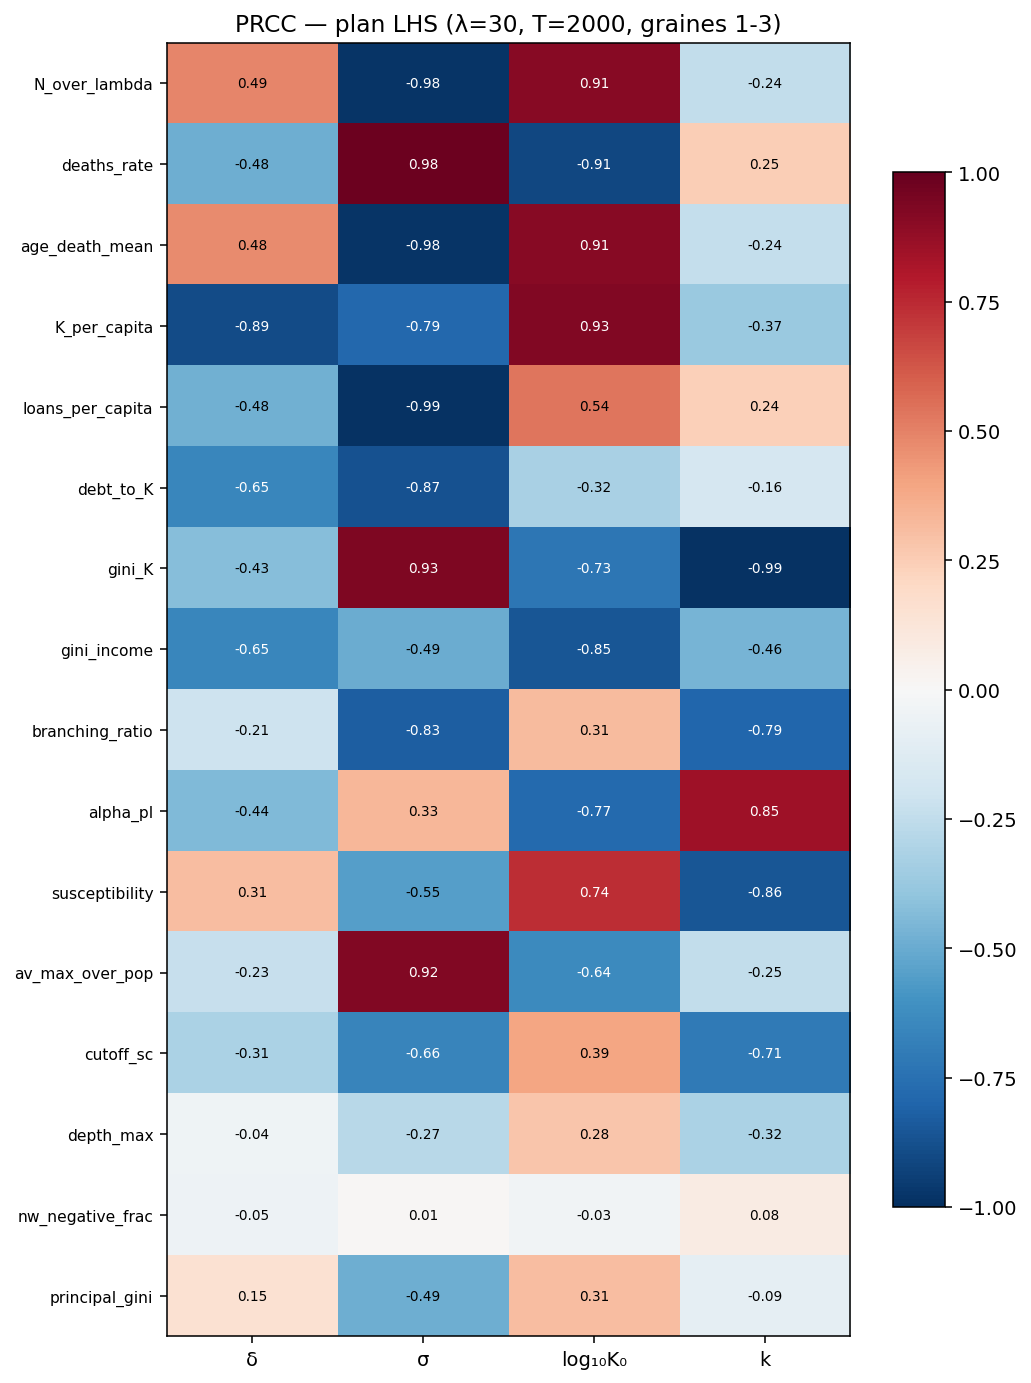
\includegraphics[width=0.78\textwidth]{lhs_prcc.png}
\caption{Corrélations de rang partielles (PRCC) entre les quatre
paramètres microscopiques et les métriques de réponse, sur le plan LHS.
Chaque case donne la corrélation partielle de rang, les autres
paramètres étant tenus fixes.}
\label{fig:lhs-prcc}
\end{figure}

Faits et inférences principaux (figure~\ref{fig:lhs-prcc}, table
\code{results/summary/lhs\_screening.csv}) :

\begin{itemize}
\item \textbf{Prédictibilité.} Les surfaces quadratiques prédisent hors
  échantillon $R^2_{\mathrm{CV}}=0{,}84$--$1{,}00$ pour treize des seize
  métriques : les réponses sont lisses et bien capturées par quatre
  paramètres, leurs carrés et leurs interactions. Exceptions :
  profondeur maximale ($R^2_{\mathrm{CV}}=0{,}09$ — extrême dominé par le
  bruit), coupure $s_c$ ($0{,}77$) et Gini des principaux ($0{,}70$).
\item \textbf{Partage des rôles.} La démographie ($N/\lambda$, taux de
  mortalité, âge au décès) est gouvernée par $\sigma$ (PRCC $\mp0{,}98$)
  puis $K_0$ ($\pm0{,}91$), $\delta$ ($\pm0{,}49$), $k$ faible
  ($\mp0{,}25$). Les inégalités de capital sont gouvernées par $k$
  (PRCC $-0{,}99$) et $\sigma$ ($+0{,}93$). La statistique des
  avalanches ($\hat\alpha$, susceptibilité, coupure) est co-gouvernée
  par $k$ (PRCC $+0{,}85$, $-0{,}86$, $-0{,}71$) et $K_0$/$\sigma$ ; le
  rapport de branchement par $\sigma$ ($-0{,}83$) et $k$ ($-0{,}79$).
  L'échelle du capital individuel est gouvernée par $\delta$
  ($-0{,}89$) et $K_0$ ($+0{,}93$).
\item \textbf{$\delta$ est partout secondaire hors échelle du capital} :
  ses PRCC sur la propagation restent modestes ($-0{,}21$ sur $b$,
  $-0{,}44$ sur $\hat\alpha$) alors qu'il contrôle fortement
  $K$ par tête et la dette/capital — cohérent avec l'hypothèse « échelle »
  issue de l'OAT.
\item \textbf{Variabilité stochastique.} La part de variance intra-point
  (graines) est $\le9\,\%$ pour treize métriques sur seize
  ($\le0{,}2\,\%$ en démographie) ; elle atteint $17\,\%$ pour la
  coupure et $72\,\%$ pour la profondeur maximale, qui ne devra être
  interprétée qu'avec les cinq graines confirmatoires. La fraction
  d'entités survivantes à valeur nette négative est structurellement
  nulle (variance nulle) : la phase de faillites élimine par
  construction toute valeur nette négative — contrôle de cohérence
  du moteur plutôt que métrique de réponse.
\item \textbf{Non-linéarités.} L'écart entre $R^2$ linéaire et
  $R^2_{\mathrm{CV}}$ quadratique (p.~ex. $0{,}85\to0{,}98$ pour
  $N/\lambda$, $0{,}72\to0{,}90$ pour le Gini de $K$, $0{,}73\to0{,}86$
  pour $b$) confirme les courbures vues en OAT (convexité en $\sigma$,
  saturation en $K_0$), sans invalider la hiérarchie ci-dessus.
\end{itemize}

Ces analyses sont exploratoires : elles hiérarchisent et sélectionnent,
la quantification finale revient à la phase confirmatoire.

\section{Décisions pour la suite de la campagne}
\label{sec:decisions}

Décisions arrêtées à l'issue de l'exploration, conformément aux règles
de passage du protocole (les choix ci-dessous s'appuient sur les
analyses exploratoires étiquetées comme telles) :

\subsection{Coupes bidimensionnelles retenues}

\begin{enumerate}
\item $\boldsymbol{\sigma\times k}$ : $\sigma\in\{0{,}05$--$0{,}50\}$
  (8 niveaux resserrés autour de la zone de transition) $\times$
  $k\in\{2,3,4,6,10\}$. Justification : ce sont les deux moteurs
  co-dominants de la propagation ($b$, $\hat\alpha$, susceptibilité) et
  des inégalités ; la coupe teste si la position et la raideur de la
  transition en $\sigma$ dépendent de $k$ (interaction).
\item $\boldsymbol{\sigma\times\delta}$ : mêmes niveaux de $\sigma$
  $\times$ $\delta\in\{0{,}02;0{,}035;0{,}05;0{,}07;0{,}10\}$.
  Justification : caractériser la crête non monotone de la
  dette/capital (maximum vers $\sigma\simeq0{,}15$--$0{,}2$) et tester
  l'hypothèse « $\delta$ = échelle pure » à tout $\sigma$ (si elle
  tient, les effets de $\delta$ sur la propagation restent faibles le
  long de toute la coupe).
\end{enumerate}

Graines $\{1,2,3\}$, $T=2000$, écriture minimale ; cellules déjà
exécutées (OAT) réutilisées par identifiant.

\subsection{Cellules confirmatoires}

$T=4000$, graines $\{11,\dots,15\}$ (disjointes de l'exploration),
instantanés périodiques tous les 100 pas, versées dans Simulation Lab et
marquées à conserver :

\begin{center}
\begin{tabularx}{\textwidth}{@{}lX@{}}
\toprule
Cellule & Motif \\
\midrule
référence $\lambda=10$ & lien avec la baseline historique du modèle \\
centre $\lambda=30$ & point d'ancrage de toute la campagne \\
$\lambda=100$ & scaling de taille (susceptibilité, coupure, maximum) \\
$\sigma=0$ & régime corrélé limite ($b\simeq0{,}65$) \\
$\sigma=0{,}10$ & zone de transition (pente maximale des réponses) \\
$\sigma=0{,}50$ & régime à vies courtes \\
$\delta=0{,}02$ et $\delta=0{,}10$ & test apparié de l'hypothèse
« échelle » \\
$K_0=5$ et $K_0=100$ & bornes du levier démographique log-linéaire \\
$k=2$ et $k=10$ & bornes du levier inégalités/statistique fine \\
$\lambda=2,\ \sigma=0{,}25$ & probabilité d'extinction initiale
($e^{-\lambda}$), 10 graines \\
\bottomrule
\end{tabularx}
\end{center}

S'y ajouteront, après dépouillement des coupes, une à deux cellules
d'interaction si un croisement qualitatif est détecté (règle du
protocole : encadrement des frontières par paires). Critères de
confirmation : signe et ordre de grandeur du contraste apparié
préservés, intervalle à 95\,\% excluant zéro, insensibilité aux burn-ins
$T/8$--$T/2$ et cohérence entre demi-fenêtres.

\subsection{Diagnostic \code{pop\_max}}

Aucune cellule n'a atteint le garde-fou à ce stade : le diagnostic
obligatoire du protocole est sans objet sur l'exploration ; il sera
réexécuté sur les runs confirmatoires ($T=4000$) et rapporté au rapport
final. Le vocabulaire « explosion » du moteur n'a jamais été employé
pour classer un run.

\subsection{Bornes et budget révisés}

Les plages initiales sont reconduites sans révision (section
\ref{sec:pilotes}). Budget consommé par l'exploration (benchmark,
pilotes, sondes, OAT, carte d'extinction, LHS) : 340 runs, zéro échec,
7{,}8\,h CPU, 3{,}65\,Go (chiffres agrégés depuis les manifestes).
Budget restant estimé pour coupes 2D + confirmation :
$\approx245$ runs, $\approx10$--$12$\,h CPU — dans l'enveloppe du
protocole.

\appendix

\section{Traçabilité des cellules citées}
\label{sec:annexe}

La table ci-dessous liste les 355 entrées de plan de la phase
exploratoire (340 runs distincts : une cellule partagée par deux plans
apparaît sous chacun). Toutes les figures et valeurs de ce rapport en
sont issues ; aucun run n'a été exclu.

% Annexe générée par scripts/make_annexe.py — ne pas éditer à la main.
{\small
\begin{longtable}{@{}llrrrrrrrl@{}}
\toprule
run\_id & plan & $\lambda$ & $\delta$ & $\sigma$ & $K_0$ & $k$ & graine & $T$ & statut \\
\midrule
\endhead
\code{m4b\_797485073afe} & benchmark & 10 & 0.05 & 0.25 & 25 & 3 & 0 & 2000 & ok \\
\code{m4b\_8efd385078ae} & benchmark & 30 & 0.05 & 0.25 & 25 & 3 & 0 & 2000 & ok \\
\code{m4b\_392895f517cd} & benchmark & 100 & 0.05 & 0.25 & 25 & 3 & 0 & 2000 & ok \\
\code{m4b\_2cb7bc83f1d9} & benchmark & 30 & 0.05 & 0.25 & 25 & 3 & 0 & 2000 & ok \\
\code{m4b\_04c4cd570599} & benchmark & 10 & 0.02 & 0.1 & 25 & 3 & 0 & 2000 & ok \\
\code{m4b\_36486750246d} & benchmark & 10 & 0.05 & 0.25 & 25 & 3 & 0 & 2000 & ok \\
\code{m4b\_f1f11729d707} & pilotes & 30 & 0.02 & 0.1 & 25 & 3 & 1 & 2000 & ok \\
\code{m4b\_63b4b58b5c5e} & pilotes & 30 & 0.02 & 0.1 & 25 & 3 & 2 & 2000 & ok \\
\code{m4b\_7ff8a4b9c628} & pilotes & 30 & 0.02 & 0.5 & 25 & 3 & 1 & 2000 & ok \\
\code{m4b\_0b15f46fa1df} & pilotes & 30 & 0.02 & 0.5 & 25 & 3 & 2 & 2000 & ok \\
\code{m4b\_c5dd2c6050e7} & pilotes & 30 & 0.1 & 0.1 & 25 & 3 & 1 & 2000 & ok \\
\code{m4b\_2180a4bc480e} & pilotes & 30 & 0.1 & 0.1 & 25 & 3 & 2 & 2000 & ok \\
\code{m4b\_83524c6aac7c} & pilotes & 30 & 0.1 & 0.5 & 25 & 3 & 1 & 2000 & ok \\
\code{m4b\_c032337f5278} & pilotes & 30 & 0.1 & 0.5 & 25 & 3 & 2 & 2000 & ok \\
\code{m4b\_35a10e8501c4} & pilotes & 30 & 0.05 & 0.25 & 5 & 3 & 1 & 2000 & ok \\
\code{m4b\_a8039a7bf647} & pilotes & 30 & 0.05 & 0.25 & 5 & 3 & 2 & 2000 & ok \\
\code{m4b\_070fbcacbeda} & pilotes & 30 & 0.05 & 0.25 & 100 & 3 & 1 & 2000 & ok \\
\code{m4b\_73aa94bd63b4} & pilotes & 30 & 0.05 & 0.25 & 100 & 3 & 2 & 2000 & ok \\
\code{m4b\_4152360a697e} & pilotes & 30 & 0.05 & 0.25 & 25 & 2 & 1 & 2000 & ok \\
\code{m4b\_76ee2b65c2bd} & pilotes & 30 & 0.05 & 0.25 & 25 & 2 & 2 & 2000 & ok \\
\code{m4b\_815693ccb3ee} & pilotes & 30 & 0.05 & 0.25 & 25 & 10 & 1 & 2000 & ok \\
\code{m4b\_6155b9db63b7} & pilotes & 30 & 0.05 & 0.25 & 25 & 10 & 2 & 2000 & ok \\
\code{m4b\_4389d08d5eef} & pilotes & 30 & 0.05 & 0 & 25 & 3 & 1 & 2000 & ok \\
\code{m4b\_334b58e2a70f} & pilotes & 30 & 0.05 & 0 & 25 & 3 & 2 & 2000 & ok \\
\code{m4b\_d9ad462f97e3} & pilotes & 30 & 0.05 & 0 & 25 & 2 & 1 & 2000 & ok \\
\code{m4b\_8614a4e0fa49} & pilotes & 30 & 0.05 & 0 & 25 & 2 & 2 & 2000 & ok \\
\code{m4b\_8d72e0e2fb28} & pilotes & 30 & 0.02 & 0 & 25 & 3 & 1 & 2000 & ok \\
\code{m4b\_d4dfdc238338} & pilotes & 30 & 0.02 & 0 & 25 & 3 & 2 & 2000 & ok \\
\code{m4b\_223ee698ee8a} & pilotes & 30 & 0.05 & 0.25 & 25 & 3 & 1 & 2000 & ok \\
\code{m4b\_9433691bedb8} & pilotes & 30 & 0.05 & 0.25 & 25 & 3 & 2 & 2000 & ok \\
\code{m4b\_0ca44bdda123} & pilotes & 30 & 0.1 & 0.5 & 5 & 3 & 1 & 2000 & ok \\
\code{m4b\_5bc5958dd40b} & pilotes & 30 & 0.1 & 0.5 & 5 & 3 & 2 & 2000 & ok \\
\code{m4b\_3373fcbcc8a5} & pilotes & 30 & 0.05 & 0.25 & 25 & 3 & 1 & 4000 & ok \\
\code{m4b\_225424622d91} & pilotes & 30 & 0.05 & 0.25 & 25 & 3 & 2 & 4000 & ok \\
\code{m4b\_4e761d701121} & pilotes & 30 & 0.02 & 0.1 & 25 & 3 & 1 & 8000 & ok \\
\code{m4b\_8c24588f6433} & pilotes & 100 & 0.02 & 0.1 & 25 & 3 & 1 & 2000 & ok \\
\code{m4b\_7e7dad60452f} & pilotes2 & 30 & 0.05 & 0.6 & 25 & 3 & 1 & 2000 & ok \\
\code{m4b\_a43d69c1d859} & pilotes2 & 30 & 0.05 & 0.6 & 25 & 3 & 2 & 2000 & ok \\
\code{m4b\_719411d80c90} & pilotes2 & 30 & 0.05 & 0.7 & 25 & 3 & 1 & 2000 & ok \\
\code{m4b\_b254dcc3b896} & pilotes2 & 30 & 0.05 & 0.7 & 25 & 3 & 2 & 2000 & ok \\
\code{m4b\_9644f4000a16} & pilotes2 & 30 & 0.05 & 0.85 & 25 & 3 & 1 & 2000 & ok \\
\code{m4b\_bd2ccb4f50b3} & pilotes2 & 30 & 0.05 & 0.85 & 25 & 3 & 2 & 2000 & ok \\
\code{m4b\_e70a79d129ed} & pilotes2 & 30 & 0.05 & 1 & 25 & 3 & 1 & 2000 & ok \\
\code{m4b\_b275a90d600c} & pilotes2 & 30 & 0.05 & 1 & 25 & 3 & 2 & 2000 & ok \\
\code{m4b\_7f5be71bde33} & pilotes2 & 30 & 0.01 & 0.05 & 25 & 3 & 1 & 2000 & ok \\
\code{m4b\_7690fbf4f754} & pilotes2 & 30 & 0.01 & 0.05 & 25 & 3 & 2 & 2000 & ok \\
\code{m4b\_e34e64d8e486} & pilotes2 & 30 & 0.01 & 0.25 & 25 & 3 & 1 & 2000 & ok \\
\code{m4b\_bf8b7868a980} & pilotes2 & 30 & 0.01 & 0.25 & 25 & 3 & 2 & 2000 & ok \\
\code{m4b\_2db90273aff4} & pilotes2 & 30 & 0.05 & 0.25 & 2 & 3 & 1 & 2000 & ok \\
\code{m4b\_9906d8cc2c20} & pilotes2 & 30 & 0.05 & 0.25 & 2 & 3 & 2 & 2000 & ok \\
\code{m4b\_5065ba3bf84e} & pilotes2 & 30 & 0.05 & 0.25 & 200 & 3 & 1 & 2000 & ok \\
\code{m4b\_5c72d7fe2ae0} & pilotes2 & 30 & 0.05 & 0.25 & 200 & 3 & 2 & 2000 & ok \\
\code{m4b\_99f85acb771b} & oat & 30 & 0.02 & 0.25 & 25 & 3 & 1 & 2000 & ok \\
\code{m4b\_6f10c4ffdf3f} & oat & 30 & 0.02 & 0.25 & 25 & 3 & 2 & 2000 & ok \\
\code{m4b\_cbf510d44807} & oat & 30 & 0.02 & 0.25 & 25 & 3 & 3 & 2000 & ok \\
\code{m4b\_7e48d343025a} & oat & 30 & 0.03 & 0.25 & 25 & 3 & 1 & 2000 & ok \\
\code{m4b\_f9736ede0c29} & oat & 30 & 0.03 & 0.25 & 25 & 3 & 2 & 2000 & ok \\
\code{m4b\_6e9d00e9fbfe} & oat & 30 & 0.03 & 0.25 & 25 & 3 & 3 & 2000 & ok \\
\code{m4b\_223ee698ee8a} & oat & 30 & 0.05 & 0.25 & 25 & 3 & 1 & 2000 & ok \\
\code{m4b\_9433691bedb8} & oat & 30 & 0.05 & 0.25 & 25 & 3 & 2 & 2000 & ok \\
\code{m4b\_1d87c9ae13e4} & oat & 30 & 0.05 & 0.25 & 25 & 3 & 3 & 2000 & ok \\
\code{m4b\_44e7b6d9479c} & oat & 30 & 0.07 & 0.25 & 25 & 3 & 1 & 2000 & ok \\
\code{m4b\_9c969e4e337c} & oat & 30 & 0.07 & 0.25 & 25 & 3 & 2 & 2000 & ok \\
\code{m4b\_f0eaa06cc865} & oat & 30 & 0.07 & 0.25 & 25 & 3 & 3 & 2000 & ok \\
\code{m4b\_40ab5c70c607} & oat & 30 & 0.1 & 0.25 & 25 & 3 & 1 & 2000 & ok \\
\code{m4b\_9355e219bada} & oat & 30 & 0.1 & 0.25 & 25 & 3 & 2 & 2000 & ok \\
\code{m4b\_c50e5463b057} & oat & 30 & 0.1 & 0.25 & 25 & 3 & 3 & 2000 & ok \\
\code{m4b\_4389d08d5eef} & oat & 30 & 0.05 & 0 & 25 & 3 & 1 & 2000 & ok \\
\code{m4b\_334b58e2a70f} & oat & 30 & 0.05 & 0 & 25 & 3 & 2 & 2000 & ok \\
\code{m4b\_16e9ffc35a50} & oat & 30 & 0.05 & 0 & 25 & 3 & 3 & 2000 & ok \\
\code{m4b\_1b8e7e58a7d1} & oat & 30 & 0.05 & 0.1 & 25 & 3 & 1 & 2000 & ok \\
\code{m4b\_a265a0190ae2} & oat & 30 & 0.05 & 0.1 & 25 & 3 & 2 & 2000 & ok \\
\code{m4b\_1275f4990c98} & oat & 30 & 0.05 & 0.1 & 25 & 3 & 3 & 2000 & ok \\
\code{m4b\_923b5e0a754c} & oat & 30 & 0.05 & 0.15 & 25 & 3 & 1 & 2000 & ok \\
\code{m4b\_be4ae4164d04} & oat & 30 & 0.05 & 0.15 & 25 & 3 & 2 & 2000 & ok \\
\code{m4b\_1402884dc872} & oat & 30 & 0.05 & 0.15 & 25 & 3 & 3 & 2000 & ok \\
\code{m4b\_f3530dbcf367} & oat & 30 & 0.05 & 0.2 & 25 & 3 & 1 & 2000 & ok \\
\code{m4b\_83ce80c2bd57} & oat & 30 & 0.05 & 0.2 & 25 & 3 & 2 & 2000 & ok \\
\code{m4b\_9887e01d6cff} & oat & 30 & 0.05 & 0.2 & 25 & 3 & 3 & 2000 & ok \\
\code{m4b\_aa8c18f6b827} & oat & 30 & 0.05 & 0.325 & 25 & 3 & 1 & 2000 & ok \\
\code{m4b\_63fc88093f48} & oat & 30 & 0.05 & 0.325 & 25 & 3 & 2 & 2000 & ok \\
\code{m4b\_37e927b1de27} & oat & 30 & 0.05 & 0.325 & 25 & 3 & 3 & 2000 & ok \\
\code{m4b\_3ddd0930487d} & oat & 30 & 0.05 & 0.4 & 25 & 3 & 1 & 2000 & ok \\
\code{m4b\_74004546d4de} & oat & 30 & 0.05 & 0.4 & 25 & 3 & 2 & 2000 & ok \\
\code{m4b\_6de962cbe8c9} & oat & 30 & 0.05 & 0.4 & 25 & 3 & 3 & 2000 & ok \\
\code{m4b\_cb087c61e004} & oat & 30 & 0.05 & 0.5 & 25 & 3 & 1 & 2000 & ok \\
\code{m4b\_23acad9dae6f} & oat & 30 & 0.05 & 0.5 & 25 & 3 & 2 & 2000 & ok \\
\code{m4b\_d54308beb42a} & oat & 30 & 0.05 & 0.5 & 25 & 3 & 3 & 2000 & ok \\
\code{m4b\_35a10e8501c4} & oat & 30 & 0.05 & 0.25 & 5 & 3 & 1 & 2000 & ok \\
\code{m4b\_a8039a7bf647} & oat & 30 & 0.05 & 0.25 & 5 & 3 & 2 & 2000 & ok \\
\code{m4b\_39343567e1f9} & oat & 30 & 0.05 & 0.25 & 5 & 3 & 3 & 2000 & ok \\
\code{m4b\_c602a838a7f1} & oat & 30 & 0.05 & 0.25 & 10 & 3 & 1 & 2000 & ok \\
\code{m4b\_d5227166331c} & oat & 30 & 0.05 & 0.25 & 10 & 3 & 2 & 2000 & ok \\
\code{m4b\_5f4c83d1cc97} & oat & 30 & 0.05 & 0.25 & 10 & 3 & 3 & 2000 & ok \\
\code{m4b\_0ab9802382e9} & oat & 30 & 0.05 & 0.25 & 50 & 3 & 1 & 2000 & ok \\
\code{m4b\_cdf5d6a63b10} & oat & 30 & 0.05 & 0.25 & 50 & 3 & 2 & 2000 & ok \\
\code{m4b\_c6b2b42aefee} & oat & 30 & 0.05 & 0.25 & 50 & 3 & 3 & 2000 & ok \\
\code{m4b\_070fbcacbeda} & oat & 30 & 0.05 & 0.25 & 100 & 3 & 1 & 2000 & ok \\
\code{m4b\_73aa94bd63b4} & oat & 30 & 0.05 & 0.25 & 100 & 3 & 2 & 2000 & ok \\
\code{m4b\_f5d52a671696} & oat & 30 & 0.05 & 0.25 & 100 & 3 & 3 & 2000 & ok \\
\code{m4b\_4152360a697e} & oat & 30 & 0.05 & 0.25 & 25 & 2 & 1 & 2000 & ok \\
\code{m4b\_76ee2b65c2bd} & oat & 30 & 0.05 & 0.25 & 25 & 2 & 2 & 2000 & ok \\
\code{m4b\_1670f6a5f468} & oat & 30 & 0.05 & 0.25 & 25 & 2 & 3 & 2000 & ok \\
\code{m4b\_f85ef5506838} & oat & 30 & 0.05 & 0.25 & 25 & 4 & 1 & 2000 & ok \\
\code{m4b\_ea1688044052} & oat & 30 & 0.05 & 0.25 & 25 & 4 & 2 & 2000 & ok \\
\code{m4b\_23e65c27433b} & oat & 30 & 0.05 & 0.25 & 25 & 4 & 3 & 2000 & ok \\
\code{m4b\_ae520266d772} & oat & 30 & 0.05 & 0.25 & 25 & 6 & 1 & 2000 & ok \\
\code{m4b\_edfaf765def4} & oat & 30 & 0.05 & 0.25 & 25 & 6 & 2 & 2000 & ok \\
\code{m4b\_1115f794fa8e} & oat & 30 & 0.05 & 0.25 & 25 & 6 & 3 & 2000 & ok \\
\code{m4b\_815693ccb3ee} & oat & 30 & 0.05 & 0.25 & 25 & 10 & 1 & 2000 & ok \\
\code{m4b\_6155b9db63b7} & oat & 30 & 0.05 & 0.25 & 25 & 10 & 2 & 2000 & ok \\
\code{m4b\_111f5ff3a21d} & oat & 30 & 0.05 & 0.25 & 25 & 10 & 3 & 2000 & ok \\
\code{m4b\_02364a291262} & oat & 10 & 0.05 & 0.25 & 25 & 3 & 1 & 2000 & ok \\
\code{m4b\_d641da597a6d} & oat & 10 & 0.05 & 0.25 & 25 & 3 & 2 & 2000 & ok \\
\code{m4b\_0d5cdd2d0b98} & oat & 10 & 0.05 & 0.25 & 25 & 3 & 3 & 2000 & ok \\
\code{m4b\_7b9b4988f289} & oat & 100 & 0.05 & 0.25 & 25 & 3 & 1 & 2000 & ok \\
\code{m4b\_b4bacbb71e13} & oat & 100 & 0.05 & 0.25 & 25 & 3 & 2 & 2000 & ok \\
\code{m4b\_97c523ee360f} & oat & 100 & 0.05 & 0.25 & 25 & 3 & 3 & 2000 & ok \\
\code{m4b\_4ae10eca1d55} & lambda\_ext & 1 & 0.05 & 0.25 & 25 & 3 & 1 & 2000 & ok \\
\code{m4b\_5a41f992ac5d} & lambda\_ext & 1 & 0.05 & 0.25 & 25 & 3 & 2 & 2000 & extinction \\
\code{m4b\_d0636ba0350b} & lambda\_ext & 1 & 0.05 & 0.25 & 25 & 3 & 3 & 2000 & extinction \\
\code{m4b\_5f27c0e30e91} & lambda\_ext & 1 & 0.05 & 0.5 & 25 & 3 & 1 & 2000 & ok \\
\code{m4b\_eb78551dd21a} & lambda\_ext & 1 & 0.05 & 0.5 & 25 & 3 & 2 & 2000 & extinction \\
\code{m4b\_e42400705557} & lambda\_ext & 1 & 0.05 & 0.5 & 25 & 3 & 3 & 2000 & extinction \\
\code{m4b\_eef15617eaf0} & lambda\_ext & 1 & 0.05 & 1 & 25 & 3 & 1 & 2000 & ok \\
\code{m4b\_42731353455a} & lambda\_ext & 1 & 0.05 & 1 & 25 & 3 & 2 & 2000 & extinction \\
\code{m4b\_1749ae4ecc0c} & lambda\_ext & 1 & 0.05 & 1 & 25 & 3 & 3 & 2000 & extinction \\
\code{m4b\_360db3e7fe18} & lambda\_ext & 2 & 0.05 & 0.25 & 25 & 3 & 1 & 2000 & ok \\
\code{m4b\_aaeb331c6434} & lambda\_ext & 2 & 0.05 & 0.25 & 25 & 3 & 2 & 2000 & ok \\
\code{m4b\_c1e0f7349e8b} & lambda\_ext & 2 & 0.05 & 0.25 & 25 & 3 & 3 & 2000 & extinction \\
\code{m4b\_acabab625d76} & lambda\_ext & 2 & 0.05 & 0.5 & 25 & 3 & 1 & 2000 & ok \\
\code{m4b\_c16b8914a4f7} & lambda\_ext & 2 & 0.05 & 0.5 & 25 & 3 & 2 & 2000 & ok \\
\code{m4b\_d28af555ed5e} & lambda\_ext & 2 & 0.05 & 0.5 & 25 & 3 & 3 & 2000 & extinction \\
\code{m4b\_aec8f19b907a} & lambda\_ext & 2 & 0.05 & 1 & 25 & 3 & 1 & 2000 & ok \\
\code{m4b\_dc71514caed4} & lambda\_ext & 2 & 0.05 & 1 & 25 & 3 & 2 & 2000 & ok \\
\code{m4b\_23e5de395bac} & lambda\_ext & 2 & 0.05 & 1 & 25 & 3 & 3 & 2000 & extinction \\
\code{m4b\_6e74dee0e7af} & lambda\_ext & 3 & 0.05 & 0.25 & 25 & 3 & 1 & 2000 & ok \\
\code{m4b\_c6953fefaa0c} & lambda\_ext & 3 & 0.05 & 0.25 & 25 & 3 & 2 & 2000 & ok \\
\code{m4b\_55f9d4efb355} & lambda\_ext & 3 & 0.05 & 0.25 & 25 & 3 & 3 & 2000 & ok \\
\code{m4b\_c644dbf2badf} & lambda\_ext & 3 & 0.05 & 0.5 & 25 & 3 & 1 & 2000 & ok \\
\code{m4b\_c099d364599a} & lambda\_ext & 3 & 0.05 & 0.5 & 25 & 3 & 2 & 2000 & ok \\
\code{m4b\_e7743f20cccd} & lambda\_ext & 3 & 0.05 & 0.5 & 25 & 3 & 3 & 2000 & ok \\
\code{m4b\_723130951bb4} & lambda\_ext & 3 & 0.05 & 1 & 25 & 3 & 1 & 2000 & ok \\
\code{m4b\_6330f21dfefd} & lambda\_ext & 3 & 0.05 & 1 & 25 & 3 & 2 & 2000 & ok \\
\code{m4b\_514da7d6a2e4} & lambda\_ext & 3 & 0.05 & 1 & 25 & 3 & 3 & 2000 & ok \\
\code{m4b\_d3b9b8c8667b} & lambda\_ext & 5 & 0.05 & 0.25 & 25 & 3 & 1 & 2000 & ok \\
\code{m4b\_0d777961e5bb} & lambda\_ext & 5 & 0.05 & 0.25 & 25 & 3 & 2 & 2000 & ok \\
\code{m4b\_562c1073c741} & lambda\_ext & 5 & 0.05 & 0.25 & 25 & 3 & 3 & 2000 & ok \\
\code{m4b\_fdf23a819932} & lambda\_ext & 5 & 0.05 & 0.5 & 25 & 3 & 1 & 2000 & ok \\
\code{m4b\_c728c089612e} & lambda\_ext & 5 & 0.05 & 0.5 & 25 & 3 & 2 & 2000 & ok \\
\code{m4b\_b1130d8ea8d9} & lambda\_ext & 5 & 0.05 & 0.5 & 25 & 3 & 3 & 2000 & ok \\
\code{m4b\_e79c17620076} & lambda\_ext & 5 & 0.05 & 1 & 25 & 3 & 1 & 2000 & ok \\
\code{m4b\_26193eb96fdf} & lambda\_ext & 5 & 0.05 & 1 & 25 & 3 & 2 & 2000 & ok \\
\code{m4b\_14ee09558ba7} & lambda\_ext & 5 & 0.05 & 1 & 25 & 3 & 3 & 2000 & ok \\
\code{m4b\_02364a291262} & lambda\_ext & 10 & 0.05 & 0.25 & 25 & 3 & 1 & 2000 & ok \\
\code{m4b\_d641da597a6d} & lambda\_ext & 10 & 0.05 & 0.25 & 25 & 3 & 2 & 2000 & ok \\
\code{m4b\_0d5cdd2d0b98} & lambda\_ext & 10 & 0.05 & 0.25 & 25 & 3 & 3 & 2000 & ok \\
\code{m4b\_b49cffd55b0f} & lambda\_ext & 10 & 0.05 & 0.5 & 25 & 3 & 1 & 2000 & ok \\
\code{m4b\_c731e8b70f37} & lambda\_ext & 10 & 0.05 & 0.5 & 25 & 3 & 2 & 2000 & ok \\
\code{m4b\_3df2904671f1} & lambda\_ext & 10 & 0.05 & 0.5 & 25 & 3 & 3 & 2000 & ok \\
\code{m4b\_fcfe1e3716da} & lambda\_ext & 10 & 0.05 & 1 & 25 & 3 & 1 & 2000 & ok \\
\code{m4b\_a42e057cc023} & lambda\_ext & 10 & 0.05 & 1 & 25 & 3 & 2 & 2000 & ok \\
\code{m4b\_f700fba07e78} & lambda\_ext & 10 & 0.05 & 1 & 25 & 3 & 3 & 2000 & ok \\
\code{m4b\_39a72e3d1fc0} & lhs & 30 & 0.063858 & 0.46613 & 50.9898 & 2 & 1 & 2000 & ok \\
\code{m4b\_3ef000a5ce82} & lhs & 30 & 0.063858 & 0.46613 & 50.9898 & 2 & 2 & 2000 & ok \\
\code{m4b\_f37ff20a868e} & lhs & 30 & 0.063858 & 0.46613 & 50.9898 & 2 & 3 & 2000 & ok \\
\code{m4b\_8ef45a8437a6} & lhs & 30 & 0.075847 & 0.26608 & 32.1034 & 6 & 1 & 2000 & ok \\
\code{m4b\_56d758fb48b7} & lhs & 30 & 0.075847 & 0.26608 & 32.1034 & 6 & 2 & 2000 & ok \\
\code{m4b\_6ff9218d1d28} & lhs & 30 & 0.075847 & 0.26608 & 32.1034 & 6 & 3 & 2000 & ok \\
\code{m4b\_d1da9b24648e} & lhs & 30 & 0.065633 & 0.085048 & 78.9057 & 4 & 1 & 2000 & ok \\
\code{m4b\_23e2148df67f} & lhs & 30 & 0.065633 & 0.085048 & 78.9057 & 4 & 2 & 2000 & ok \\
\code{m4b\_a8f86933311d} & lhs & 30 & 0.065633 & 0.085048 & 78.9057 & 4 & 3 & 2000 & ok \\
\code{m4b\_ed254aa15b83} & lhs & 30 & 0.061769 & 0.440245 & 73.8598 & 4 & 1 & 2000 & ok \\
\code{m4b\_bfc61c066ecc} & lhs & 30 & 0.061769 & 0.440245 & 73.8598 & 4 & 2 & 2000 & ok \\
\code{m4b\_8063b9bef07c} & lhs & 30 & 0.061769 & 0.440245 & 73.8598 & 4 & 3 & 2000 & ok \\
\code{m4b\_ee3dbe0f4792} & lhs & 30 & 0.098054 & 0.175738 & 14.3985 & 10 & 1 & 2000 & ok \\
\code{m4b\_a5cb3e7a7662} & lhs & 30 & 0.098054 & 0.175738 & 14.3985 & 10 & 2 & 2000 & ok \\
\code{m4b\_b3b16c3b49a3} & lhs & 30 & 0.098054 & 0.175738 & 14.3985 & 10 & 3 & 2000 & ok \\
\code{m4b\_28aaf687a56a} & lhs & 30 & 0.026947 & 0.401449 & 64.4304 & 4 & 1 & 2000 & ok \\
\code{m4b\_fe28ad64e575} & lhs & 30 & 0.026947 & 0.401449 & 64.4304 & 4 & 2 & 2000 & ok \\
\code{m4b\_9c818ece38f8} & lhs & 30 & 0.026947 & 0.401449 & 64.4304 & 4 & 3 & 2000 & ok \\
\code{m4b\_267d175cc22b} & lhs & 30 & 0.085287 & 0.190251 & 32.6411 & 3 & 1 & 2000 & ok \\
\code{m4b\_87dbd7ea78d3} & lhs & 30 & 0.085287 & 0.190251 & 32.6411 & 3 & 2 & 2000 & ok \\
\code{m4b\_e8800e499a4f} & lhs & 30 & 0.085287 & 0.190251 & 32.6411 & 3 & 3 & 2000 & ok \\
\code{m4b\_7ed96bfbafc6} & lhs & 30 & 0.067687 & 0.458375 & 47.5609 & 10 & 1 & 2000 & ok \\
\code{m4b\_319521b4b71e} & lhs & 30 & 0.067687 & 0.458375 & 47.5609 & 10 & 2 & 2000 & ok \\
\code{m4b\_4a72c158acff} & lhs & 30 & 0.067687 & 0.458375 & 47.5609 & 10 & 3 & 2000 & ok \\
\code{m4b\_c45bfa74504a} & lhs & 30 & 0.031771 & 0.42397 & 5.5741 & 6 & 1 & 2000 & ok \\
\code{m4b\_4a40a8eacda8} & lhs & 30 & 0.031771 & 0.42397 & 5.5741 & 6 & 2 & 2000 & ok \\
\code{m4b\_c76988285f78} & lhs & 30 & 0.031771 & 0.42397 & 5.5741 & 6 & 3 & 2000 & ok \\
\code{m4b\_ffb62fa7ba7e} & lhs & 30 & 0.025186 & 0.121166 & 9.9798 & 6 & 1 & 2000 & ok \\
\code{m4b\_0a28b4c2e4d1} & lhs & 30 & 0.025186 & 0.121166 & 9.9798 & 6 & 2 & 2000 & ok \\
\code{m4b\_a0562505b8f0} & lhs & 30 & 0.025186 & 0.121166 & 9.9798 & 6 & 3 & 2000 & ok \\
\code{m4b\_6d5b3cfd6226} & lhs & 30 & 0.067218 & 0.347318 & 34.526 & 2 & 1 & 2000 & ok \\
\code{m4b\_caf5b1205c7f} & lhs & 30 & 0.067218 & 0.347318 & 34.526 & 2 & 2 & 2000 & ok \\
\code{m4b\_de2b4765cd81} & lhs & 30 & 0.067218 & 0.347318 & 34.526 & 2 & 3 & 2000 & ok \\
\code{m4b\_3f058fec4979} & lhs & 30 & 0.058837 & 0.404774 & 6.9407 & 3 & 1 & 2000 & ok \\
\code{m4b\_efb76cf83d62} & lhs & 30 & 0.058837 & 0.404774 & 6.9407 & 3 & 2 & 2000 & ok \\
\code{m4b\_135f19b1ab8a} & lhs & 30 & 0.058837 & 0.404774 & 6.9407 & 3 & 3 & 2000 & ok \\
\code{m4b\_adc54cf3df23} & lhs & 30 & 0.094942 & 0.218124 & 6.6275 & 2 & 1 & 2000 & ok \\
\code{m4b\_e288eaf6af33} & lhs & 30 & 0.094942 & 0.218124 & 6.6275 & 2 & 2 & 2000 & ok \\
\code{m4b\_d71321c4c9aa} & lhs & 30 & 0.094942 & 0.218124 & 6.6275 & 2 & 3 & 2000 & ok \\
\code{m4b\_1cc788ca55b4} & lhs & 30 & 0.052282 & 0.16928 & 11.5838 & 10 & 1 & 2000 & ok \\
\code{m4b\_989bfbd1015e} & lhs & 30 & 0.052282 & 0.16928 & 11.5838 & 10 & 2 & 2000 & ok \\
\code{m4b\_ce39ab061450} & lhs & 30 & 0.052282 & 0.16928 & 11.5838 & 10 & 3 & 2000 & ok \\
\code{m4b\_124cb7934ad9} & lhs & 30 & 0.078115 & 0.064081 & 9.3816 & 3 & 1 & 2000 & ok \\
\code{m4b\_6fff694dc229} & lhs & 30 & 0.078115 & 0.064081 & 9.3816 & 3 & 2 & 2000 & ok \\
\code{m4b\_180aec48dca7} & lhs & 30 & 0.078115 & 0.064081 & 9.3816 & 3 & 3 & 2000 & ok \\
\code{m4b\_5bace300d083} & lhs & 30 & 0.023047 & 0.240842 & 5.2037 & 2 & 1 & 2000 & ok \\
\code{m4b\_fd0a45407982} & lhs & 30 & 0.023047 & 0.240842 & 5.2037 & 2 & 2 & 2000 & ok \\
\code{m4b\_061323b0834a} & lhs & 30 & 0.023047 & 0.240842 & 5.2037 & 2 & 3 & 2000 & ok \\
\code{m4b\_6ac1d242222f} & lhs & 30 & 0.089892 & 0.278599 & 8.6068 & 2 & 1 & 2000 & ok \\
\code{m4b\_33984830b4f6} & lhs & 30 & 0.089892 & 0.278599 & 8.6068 & 2 & 2 & 2000 & ok \\
\code{m4b\_bb67c9633a4c} & lhs & 30 & 0.089892 & 0.278599 & 8.6068 & 2 & 3 & 2000 & ok \\
\code{m4b\_38d605cf2be7} & lhs & 30 & 0.033098 & 0.099133 & 65.8046 & 2 & 1 & 2000 & ok \\
\code{m4b\_8bcd84a874ab} & lhs & 30 & 0.033098 & 0.099133 & 65.8046 & 2 & 2 & 2000 & ok \\
\code{m4b\_57e2d8c88af9} & lhs & 30 & 0.033098 & 0.099133 & 65.8046 & 2 & 3 & 2000 & ok \\
\code{m4b\_917275d302fc} & lhs & 30 & 0.053405 & 0.478603 & 69.7375 & 3 & 1 & 2000 & ok \\
\code{m4b\_45f67f0bbf55} & lhs & 30 & 0.053405 & 0.478603 & 69.7375 & 3 & 2 & 2000 & ok \\
\code{m4b\_208ce5781a40} & lhs & 30 & 0.053405 & 0.478603 & 69.7375 & 3 & 3 & 2000 & ok \\
\code{m4b\_909fecc30dfc} & lhs & 30 & 0.088283 & 0.053279 & 37.6723 & 2 & 1 & 2000 & ok \\
\code{m4b\_5685195e1c7a} & lhs & 30 & 0.088283 & 0.053279 & 37.6723 & 2 & 2 & 2000 & ok \\
\code{m4b\_29a6094b9ad9} & lhs & 30 & 0.088283 & 0.053279 & 37.6723 & 2 & 3 & 2000 & ok \\
\code{m4b\_76393dc9b361} & lhs & 30 & 0.049354 & 0.314858 & 9.0347 & 3 & 1 & 2000 & ok \\
\code{m4b\_da8fe6387809} & lhs & 30 & 0.049354 & 0.314858 & 9.0347 & 3 & 2 & 2000 & ok \\
\code{m4b\_d855e7c36f59} & lhs & 30 & 0.049354 & 0.314858 & 9.0347 & 3 & 3 & 2000 & ok \\
\code{m4b\_78294a671c63} & lhs & 30 & 0.096073 & 0.325641 & 47.0778 & 3 & 1 & 2000 & ok \\
\code{m4b\_8d237d8f5928} & lhs & 30 & 0.096073 & 0.325641 & 47.0778 & 3 & 2 & 2000 & ok \\
\code{m4b\_f855d5bbaddf} & lhs & 30 & 0.096073 & 0.325641 & 47.0778 & 3 & 3 & 2000 & ok \\
\code{m4b\_716a65d5c3c9} & lhs & 30 & 0.096634 & 0.118149 & 18.8551 & 6 & 1 & 2000 & ok \\
\code{m4b\_826350fb499a} & lhs & 30 & 0.096634 & 0.118149 & 18.8551 & 6 & 2 & 2000 & ok \\
\code{m4b\_f6f0bf895eb8} & lhs & 30 & 0.096634 & 0.118149 & 18.8551 & 6 & 3 & 2000 & ok \\
\code{m4b\_5d25fe0aff4e} & lhs & 30 & 0.036043 & 0.368594 & 10.7385 & 3 & 1 & 2000 & ok \\
\code{m4b\_bae5bef82f33} & lhs & 30 & 0.036043 & 0.368594 & 10.7385 & 3 & 2 & 2000 & ok \\
\code{m4b\_65bd72ec9fb3} & lhs & 30 & 0.036043 & 0.368594 & 10.7385 & 3 & 3 & 2000 & ok \\
\code{m4b\_07a6da4ff3e3} & lhs & 30 & 0.046232 & 0.434683 & 7.8702 & 10 & 1 & 2000 & ok \\
\code{m4b\_efe6ac800175} & lhs & 30 & 0.046232 & 0.434683 & 7.8702 & 10 & 2 & 2000 & ok \\
\code{m4b\_2ad6858466c9} & lhs & 30 & 0.046232 & 0.434683 & 7.8702 & 10 & 3 & 2000 & ok \\
\code{m4b\_3e1c57383ba9} & lhs & 30 & 0.086949 & 0.204272 & 61.6583 & 2 & 1 & 2000 & ok \\
\code{m4b\_3da454b89cdd} & lhs & 30 & 0.086949 & 0.204272 & 61.6583 & 2 & 2 & 2000 & ok \\
\code{m4b\_6b3a0b9058d5} & lhs & 30 & 0.086949 & 0.204272 & 61.6583 & 2 & 3 & 2000 & ok \\
\code{m4b\_8100a18e0906} & lhs & 30 & 0.041977 & 0.230304 & 85.8936 & 10 & 1 & 2000 & ok \\
\code{m4b\_de00695c3da2} & lhs & 30 & 0.041977 & 0.230304 & 85.8936 & 10 & 2 & 2000 & ok \\
\code{m4b\_85324cba4b54} & lhs & 30 & 0.041977 & 0.230304 & 85.8936 & 10 & 3 & 2000 & ok \\
\code{m4b\_686a50fab132} & lhs & 30 & 0.091404 & 0.449024 & 13.6027 & 6 & 1 & 2000 & ok \\
\code{m4b\_fd98a3a34650} & lhs & 30 & 0.091404 & 0.449024 & 13.6027 & 6 & 2 & 2000 & ok \\
\code{m4b\_dbebefd33cc8} & lhs & 30 & 0.091404 & 0.449024 & 13.6027 & 6 & 3 & 2000 & ok \\
\code{m4b\_4acb0a655cdf} & lhs & 30 & 0.082717 & 0.210107 & 8.1073 & 6 & 1 & 2000 & ok \\
\code{m4b\_a753a47db6ff} & lhs & 30 & 0.082717 & 0.210107 & 8.1073 & 6 & 2 & 2000 & ok \\
\code{m4b\_da9479c05357} & lhs & 30 & 0.082717 & 0.210107 & 8.1073 & 6 & 3 & 2000 & ok \\
\code{m4b\_f6f9333e98d4} & lhs & 30 & 0.070664 & 0.090788 & 24.0655 & 4 & 1 & 2000 & ok \\
\code{m4b\_a1a4cb27a44c} & lhs & 30 & 0.070664 & 0.090788 & 24.0655 & 4 & 2 & 2000 & ok \\
\code{m4b\_08e26181b9b7} & lhs & 30 & 0.070664 & 0.090788 & 24.0655 & 4 & 3 & 2000 & ok \\
\code{m4b\_83fc6edca183} & lhs & 30 & 0.079882 & 0.282096 & 5.3042 & 3 & 1 & 2000 & ok \\
\code{m4b\_848adb23bd81} & lhs & 30 & 0.079882 & 0.282096 & 5.3042 & 3 & 2 & 2000 & ok \\
\code{m4b\_0f9768859bfb} & lhs & 30 & 0.079882 & 0.282096 & 5.3042 & 3 & 3 & 2000 & ok \\
\code{m4b\_beb94650f82c} & lhs & 30 & 0.023752 & 0.380185 & 15.0446 & 6 & 1 & 2000 & ok \\
\code{m4b\_e481e8d34886} & lhs & 30 & 0.023752 & 0.380185 & 15.0446 & 6 & 2 & 2000 & ok \\
\code{m4b\_fdc7cdfe0a5c} & lhs & 30 & 0.023752 & 0.380185 & 15.0446 & 6 & 3 & 2000 & ok \\
\code{m4b\_397f7ab1139a} & lhs & 30 & 0.054295 & 0.102096 & 28.7243 & 6 & 1 & 2000 & ok \\
\code{m4b\_e3c1da58eea7} & lhs & 30 & 0.054295 & 0.102096 & 28.7243 & 6 & 2 & 2000 & ok \\
\code{m4b\_9c5351533fec} & lhs & 30 & 0.054295 & 0.102096 & 28.7243 & 6 & 3 & 2000 & ok \\
\code{m4b\_bd88fb610519} & lhs & 30 & 0.034538 & 0.337503 & 54.7801 & 10 & 1 & 2000 & ok \\
\code{m4b\_1440049b7414} & lhs & 30 & 0.034538 & 0.337503 & 54.7801 & 10 & 2 & 2000 & ok \\
\code{m4b\_58b3d6e4af7a} & lhs & 30 & 0.034538 & 0.337503 & 54.7801 & 10 & 3 & 2000 & ok \\
\code{m4b\_c6622bd1bcc7} & lhs & 30 & 0.047476 & 0.414513 & 27.3939 & 4 & 1 & 2000 & ok \\
\code{m4b\_a7016db69222} & lhs & 30 & 0.047476 & 0.414513 & 27.3939 & 4 & 2 & 2000 & ok \\
\code{m4b\_a1cd9abd5ecf} & lhs & 30 & 0.047476 & 0.414513 & 27.3939 & 4 & 3 & 2000 & ok \\
\code{m4b\_5914883ade3b} & lhs & 30 & 0.099749 & 0.063934 & 57.5848 & 4 & 1 & 2000 & ok \\
\code{m4b\_5a8f669b9b9f} & lhs & 30 & 0.099749 & 0.063934 & 57.5848 & 4 & 2 & 2000 & ok \\
\code{m4b\_d5519eaf19ee} & lhs & 30 & 0.099749 & 0.063934 & 57.5848 & 4 & 3 & 2000 & ok \\
\code{m4b\_72ab515dd103} & lhs & 30 & 0.020548 & 0.146925 & 39.922 & 6 & 1 & 2000 & ok \\
\code{m4b\_7b2b8215a4ae} & lhs & 30 & 0.020548 & 0.146925 & 39.922 & 6 & 2 & 2000 & ok \\
\code{m4b\_d5adf0e0e7b2} & lhs & 30 & 0.020548 & 0.146925 & 39.922 & 6 & 3 & 2000 & ok \\
\code{m4b\_dd1a9e6a4949} & lhs & 30 & 0.050234 & 0.380642 & 19.4422 & 4 & 1 & 2000 & ok \\
\code{m4b\_71948b75b25d} & lhs & 30 & 0.050234 & 0.380642 & 19.4422 & 4 & 2 & 2000 & ok \\
\code{m4b\_0ba31aabf0d5} & lhs & 30 & 0.050234 & 0.380642 & 19.4422 & 4 & 3 & 2000 & ok \\
\code{m4b\_89d26099968e} & lhs & 30 & 0.069716 & 0.223185 & 6.5325 & 4 & 1 & 2000 & ok \\
\code{m4b\_c8ff6ccd1483} & lhs & 30 & 0.069716 & 0.223185 & 6.5325 & 4 & 2 & 2000 & ok \\
\code{m4b\_c3c4fe028cd6} & lhs & 30 & 0.069716 & 0.223185 & 6.5325 & 4 & 3 & 2000 & ok \\
\code{m4b\_6614a3fc3623} & lhs & 30 & 0.030927 & 0.344401 & 12.8133 & 6 & 1 & 2000 & ok \\
\code{m4b\_6c3feae323e2} & lhs & 30 & 0.030927 & 0.344401 & 12.8133 & 6 & 2 & 2000 & ok \\
\code{m4b\_b80f334975e5} & lhs & 30 & 0.030927 & 0.344401 & 12.8133 & 6 & 3 & 2000 & ok \\
\code{m4b\_5fa6edba1233} & lhs & 30 & 0.076635 & 0.29324 & 11.6757 & 3 & 1 & 2000 & ok \\
\code{m4b\_29b7cc5fe293} & lhs & 30 & 0.076635 & 0.29324 & 11.6757 & 3 & 2 & 2000 & ok \\
\code{m4b\_abc86326a373} & lhs & 30 & 0.076635 & 0.29324 & 11.6757 & 3 & 3 & 2000 & ok \\
\code{m4b\_2112bc6141ae} & lhs & 30 & 0.028112 & 0.364769 & 81.5083 & 10 & 1 & 2000 & ok \\
\code{m4b\_087c65fa2765} & lhs & 30 & 0.028112 & 0.364769 & 81.5083 & 10 & 2 & 2000 & ok \\
\code{m4b\_24464b102be5} & lhs & 30 & 0.028112 & 0.364769 & 81.5083 & 10 & 3 & 2000 & ok \\
\code{m4b\_54cae5e4eb69} & lhs & 30 & 0.080341 & 0.194967 & 43.208 & 3 & 1 & 2000 & ok \\
\code{m4b\_cf82b687149a} & lhs & 30 & 0.080341 & 0.194967 & 43.208 & 3 & 2 & 2000 & ok \\
\code{m4b\_977541e1bd2f} & lhs & 30 & 0.080341 & 0.194967 & 43.208 & 3 & 3 & 2000 & ok \\
\code{m4b\_5029ecf757bc} & lhs & 30 & 0.073223 & 0.479162 & 42.3947 & 10 & 1 & 2000 & ok \\
\code{m4b\_cb186bbb12cd} & lhs & 30 & 0.073223 & 0.479162 & 42.3947 & 10 & 2 & 2000 & ok \\
\code{m4b\_f7748cdcc7a8} & lhs & 30 & 0.073223 & 0.479162 & 42.3947 & 10 & 3 & 2000 & ok \\
\code{m4b\_b43a28b3002f} & lhs & 30 & 0.043798 & 0.27386 & 89.4412 & 4 & 1 & 2000 & ok \\
\code{m4b\_7bb17548a177} & lhs & 30 & 0.043798 & 0.27386 & 89.4412 & 4 & 2 & 2000 & ok \\
\code{m4b\_c97098f073e0} & lhs & 30 & 0.043798 & 0.27386 & 89.4412 & 4 & 3 & 2000 & ok \\
\code{m4b\_1c4b8779ccfd} & lhs & 30 & 0.081586 & 0.151079 & 17.719 & 4 & 1 & 2000 & ok \\
\code{m4b\_f37c6b2a014a} & lhs & 30 & 0.081586 & 0.151079 & 17.719 & 4 & 2 & 2000 & ok \\
\code{m4b\_8fae2902035b} & lhs & 30 & 0.081586 & 0.151079 & 17.719 & 4 & 3 & 2000 & ok \\
\code{m4b\_f7753c3cd3e2} & lhs & 30 & 0.04006 & 0.489398 & 25.8756 & 6 & 1 & 2000 & ok \\
\code{m4b\_ec2201fa5a01} & lhs & 30 & 0.04006 & 0.489398 & 25.8756 & 6 & 2 & 2000 & ok \\
\code{m4b\_001a75064887} & lhs & 30 & 0.04006 & 0.489398 & 25.8756 & 6 & 3 & 2000 & ok \\
\code{m4b\_0100c02ae6dc} & lhs & 30 & 0.055815 & 0.420941 & 17.2064 & 3 & 1 & 2000 & ok \\
\code{m4b\_6bb477c1e709} & lhs & 30 & 0.055815 & 0.420941 & 17.2064 & 3 & 2 & 2000 & ok \\
\code{m4b\_109d9baa9827} & lhs & 30 & 0.055815 & 0.420941 & 17.2064 & 3 & 3 & 2000 & ok \\
\code{m4b\_c6c006fc5ed5} & lhs & 30 & 0.072237 & 0.247181 & 52.8085 & 2 & 1 & 2000 & ok \\
\code{m4b\_dac9fcd259b3} & lhs & 30 & 0.072237 & 0.247181 & 52.8085 & 2 & 2 & 2000 & ok \\
\code{m4b\_bf0a4b0837ee} & lhs & 30 & 0.072237 & 0.247181 & 52.8085 & 2 & 3 & 2000 & ok \\
\code{m4b\_2baa46f7f961} & lhs & 30 & 0.074581 & 0.239189 & 23.2299 & 10 & 1 & 2000 & ok \\
\code{m4b\_311fcfe6b3a8} & lhs & 30 & 0.074581 & 0.239189 & 23.2299 & 10 & 2 & 2000 & ok \\
\code{m4b\_d7890d102482} & lhs & 30 & 0.074581 & 0.239189 & 23.2299 & 10 & 3 & 2000 & ok \\
\code{m4b\_038bdecc93fb} & lhs & 30 & 0.042747 & 0.451706 & 95.4553 & 3 & 1 & 2000 & ok \\
\code{m4b\_169bf449bfb9} & lhs & 30 & 0.042747 & 0.451706 & 95.4553 & 3 & 2 & 2000 & ok \\
\code{m4b\_98e0a73bb321} & lhs & 30 & 0.042747 & 0.451706 & 95.4553 & 3 & 3 & 2000 & ok \\
\code{m4b\_ef11e8285806} & lhs & 30 & 0.092994 & 0.131713 & 37.0158 & 6 & 1 & 2000 & ok \\
\code{m4b\_2524d4560b56} & lhs & 30 & 0.092994 & 0.131713 & 37.0158 & 6 & 2 & 2000 & ok \\
\code{m4b\_5df5932ef174} & lhs & 30 & 0.092994 & 0.131713 & 37.0158 & 6 & 3 & 2000 & ok \\
\code{m4b\_45a390baaff2} & lhs & 30 & 0.029075 & 0.390801 & 15.8141 & 10 & 1 & 2000 & ok \\
\code{m4b\_b62c66aa0f8b} & lhs & 30 & 0.029075 & 0.390801 & 15.8141 & 10 & 2 & 2000 & ok \\
\code{m4b\_0d7a06c55926} & lhs & 30 & 0.029075 & 0.390801 & 15.8141 & 10 & 3 & 2000 & ok \\
\code{m4b\_100b95f9ac4a} & lhs & 30 & 0.084759 & 0.157742 & 7.3521 & 10 & 1 & 2000 & ok \\
\code{m4b\_d7030118b93e} & lhs & 30 & 0.084759 & 0.157742 & 7.3521 & 10 & 2 & 2000 & ok \\
\code{m4b\_ef0202c7d055} & lhs & 30 & 0.084759 & 0.157742 & 7.3521 & 10 & 3 & 2000 & ok \\
\code{m4b\_de2a4902f9c7} & lhs & 30 & 0.037658 & 0.135285 & 24.7389 & 2 & 1 & 2000 & ok \\
\code{m4b\_813425fac02c} & lhs & 30 & 0.037658 & 0.135285 & 24.7389 & 2 & 2 & 2000 & ok \\
\code{m4b\_2959bddea1a9} & lhs & 30 & 0.037658 & 0.135285 & 24.7389 & 2 & 3 & 2000 & ok \\
\code{m4b\_f32f73f3f632} & lhs & 30 & 0.057072 & 0.495695 & 20.6928 & 2 & 1 & 2000 & ok \\
\code{m4b\_2fb7a5285444} & lhs & 30 & 0.057072 & 0.495695 & 20.6928 & 2 & 2 & 2000 & ok \\
\code{m4b\_cdf46d8cc0da} & lhs & 30 & 0.057072 & 0.495695 & 20.6928 & 2 & 3 & 2000 & ok \\
\code{m4b\_e7b379bd7442} & lhs & 30 & 0.047773 & 0.305666 & 21.6897 & 6 & 1 & 2000 & ok \\
\code{m4b\_1fa4dd4f6ee5} & lhs & 30 & 0.047773 & 0.305666 & 21.6897 & 6 & 2 & 2000 & ok \\
\code{m4b\_124cbd4162d9} & lhs & 30 & 0.047773 & 0.305666 & 21.6897 & 6 & 3 & 2000 & ok \\
\code{m4b\_0cc9ba8b5100} & lhs & 30 & 0.060222 & 0.297793 & 29.6452 & 2 & 1 & 2000 & ok \\
\code{m4b\_b856190c5e40} & lhs & 30 & 0.060222 & 0.297793 & 29.6452 & 2 & 2 & 2000 & ok \\
\code{m4b\_0d77c8ef2572} & lhs & 30 & 0.060222 & 0.297793 & 29.6452 & 2 & 3 & 2000 & ok \\
\code{m4b\_84f108feaed4} & lhs & 30 & 0.039522 & 0.352381 & 92.6702 & 3 & 1 & 2000 & ok \\
\code{m4b\_486855b9781a} & lhs & 30 & 0.039522 & 0.352381 & 92.6702 & 3 & 2 & 2000 & ok \\
\code{m4b\_9fb0b2956ce7} & lhs & 30 & 0.039522 & 0.352381 & 92.6702 & 3 & 3 & 2000 & ok \\
\code{m4b\_a7e33fc52ad8} & lhs & 30 & 0.021462 & 0.106465 & 16.2381 & 10 & 1 & 2000 & ok \\
\code{m4b\_c9984e00c807} & lhs & 30 & 0.021462 & 0.106465 & 16.2381 & 10 & 2 & 2000 & ok \\
\code{m4b\_1eaab91ead8d} & lhs & 30 & 0.021462 & 0.106465 & 16.2381 & 10 & 3 & 2000 & ok \\
\code{m4b\_dfd45a9c87c5} & lhs & 30 & 0.058593 & 0.321352 & 6.0982 & 4 & 1 & 2000 & ok \\
\code{m4b\_59766367a4ac} & lhs & 30 & 0.058593 & 0.321352 & 6.0982 & 4 & 2 & 2000 & ok \\
\code{m4b\_42e520f71c62} & lhs & 30 & 0.058593 & 0.321352 & 6.0982 & 4 & 3 & 2000 & ok \\
\code{m4b\_91f5058fc348} & lhs & 30 & 0.036711 & 0.25851 & 10.3307 & 2 & 1 & 2000 & ok \\
\code{m4b\_682763940fec} & lhs & 30 & 0.036711 & 0.25851 & 10.3307 & 2 & 2 & 2000 & ok \\
\code{m4b\_1ab4ec997566} & lhs & 30 & 0.036711 & 0.25851 & 10.3307 & 2 & 3 & 2000 & ok \\
\code{m4b\_35c4a75a92f1} & lhs & 30 & 0.062996 & 0.177052 & 12.7042 & 4 & 1 & 2000 & ok \\
\code{m4b\_9766573f74b4} & lhs & 30 & 0.062996 & 0.177052 & 12.7042 & 4 & 2 & 2000 & ok \\
\code{m4b\_f00ffe13cbf6} & lhs & 30 & 0.062996 & 0.177052 & 12.7042 & 4 & 3 & 2000 & ok \\
\code{m4b\_13f4e72900a9} & lhs & 30 & 0.090683 & 0.076835 & 6.0014 & 4 & 1 & 2000 & ok \\
\code{m4b\_316f96c01a01} & lhs & 30 & 0.090683 & 0.076835 & 6.0014 & 4 & 2 & 2000 & ok \\
\code{m4b\_f690a315b249} & lhs & 30 & 0.090683 & 0.076835 & 6.0014 & 4 & 3 & 2000 & ok \\
\bottomrule
\end{longtable}
}

\noindent Usages par plan : \textbf{benchmark} : benchmark de coût (protocole §9) ; contrôles de neutralité ; \textbf{pilotes} : audit des plages (§3), contrôles temporels (§4), fig. pilotes ; \textbf{pilotes2} : sondes de frontière (§6.1) ; \textbf{oat} : courbes OAT (§5, fig. oat\_*) ; \textbf{lambda\_ext} : carte d'extinction (§6.2) ; \textbf{lhs} : screening global (§7, fig. lhs\_*).

\noindent Chaque run est reproductible depuis son manifeste (\path{results/runs/<run_id>/manifest.json}) : moteur \code{m4b-mini-3} (condensat \code{f3a7ce02cd9185c7}), paramètres complets, graine, options d'écriture. Les données primaires et les métriques dérivées (\path{results/metrics/<run_id>.json}) sont conservées.

\end{document}
